% Chapter Four - A Radiation Damage Simulation for the HF Detector

\chapter{A Radiation Damage Simulation for the HF Detector} \label{chapter:HFRaddam}
 This chapter describes a radiation damage software package developed inside CMSSW (Section \ref{Section:CMSSW}) release 6\_1\_2\_SLHC4\_patch2, and which has subsequently been propagated to later releases.

	\section{Introduction to HF}
		The Hadronic Forward detector is part of the HCAL system in CMS, and is designed to reconstruct jets that occur at high-$|\eta|$, close to the beam line.  The HF detector is an iron absorber/quartz fiber calorimeter.  Quartz fibers are embedded in large iron sheets;  the iron absorber creates showers of particles, and the quartz fibers are used to generate Cherenkov radiation from the showers and transmit this light to photomultiplier tubes (PMT) in a readout box near the rear of the detector.  Each iron/quartz module is referred to as a \textit{wedge}, and are stacked to create a cylinder.  See Figure \ref{figure:HFQuartz} for a view of a row of HF wedges.  Each wedge is divided into 24 \textit{towers}, see Figure \ref{figure:HFTower}.  The fibers in each tower are grouped together and read out by a single PMT.  Towers are then clustered together in software to reconstruct jets.
		
		As described in Section \ref{section:jets}, good jet reconstruction relies on the quality of the clusters available for clustering, which in turn relies on the amount of light reaching the surface of the PMT from the fibers.
		
		With the increasing energy of the LHC beam collisions, the HF detector becomes more and more relevant, as more and more interesting events occur at high-$|\eta|$.  In particular, the signature for Higgs vector boson fusion production is two high-$|eta|$ jets, well separated; perfect for HF.
		
		Therefore, it is imperative that the performance of the HF detector at high integrated luminosity is understood, as its relevance will increase with energy and luminosity, but so will its radiation exposure.
		
		In Figure \ref{fig:CMSLabelled} the HF detector is visible on either sides of the detector, near the beam line, labeled `Very Forward Calorimeter'.
	
		%%%%%%%%%%%%%%%%% HF Wedge %%%%%%%%%%%%%%%%%%%
		\begin{figure}[]
			\begin{center}
				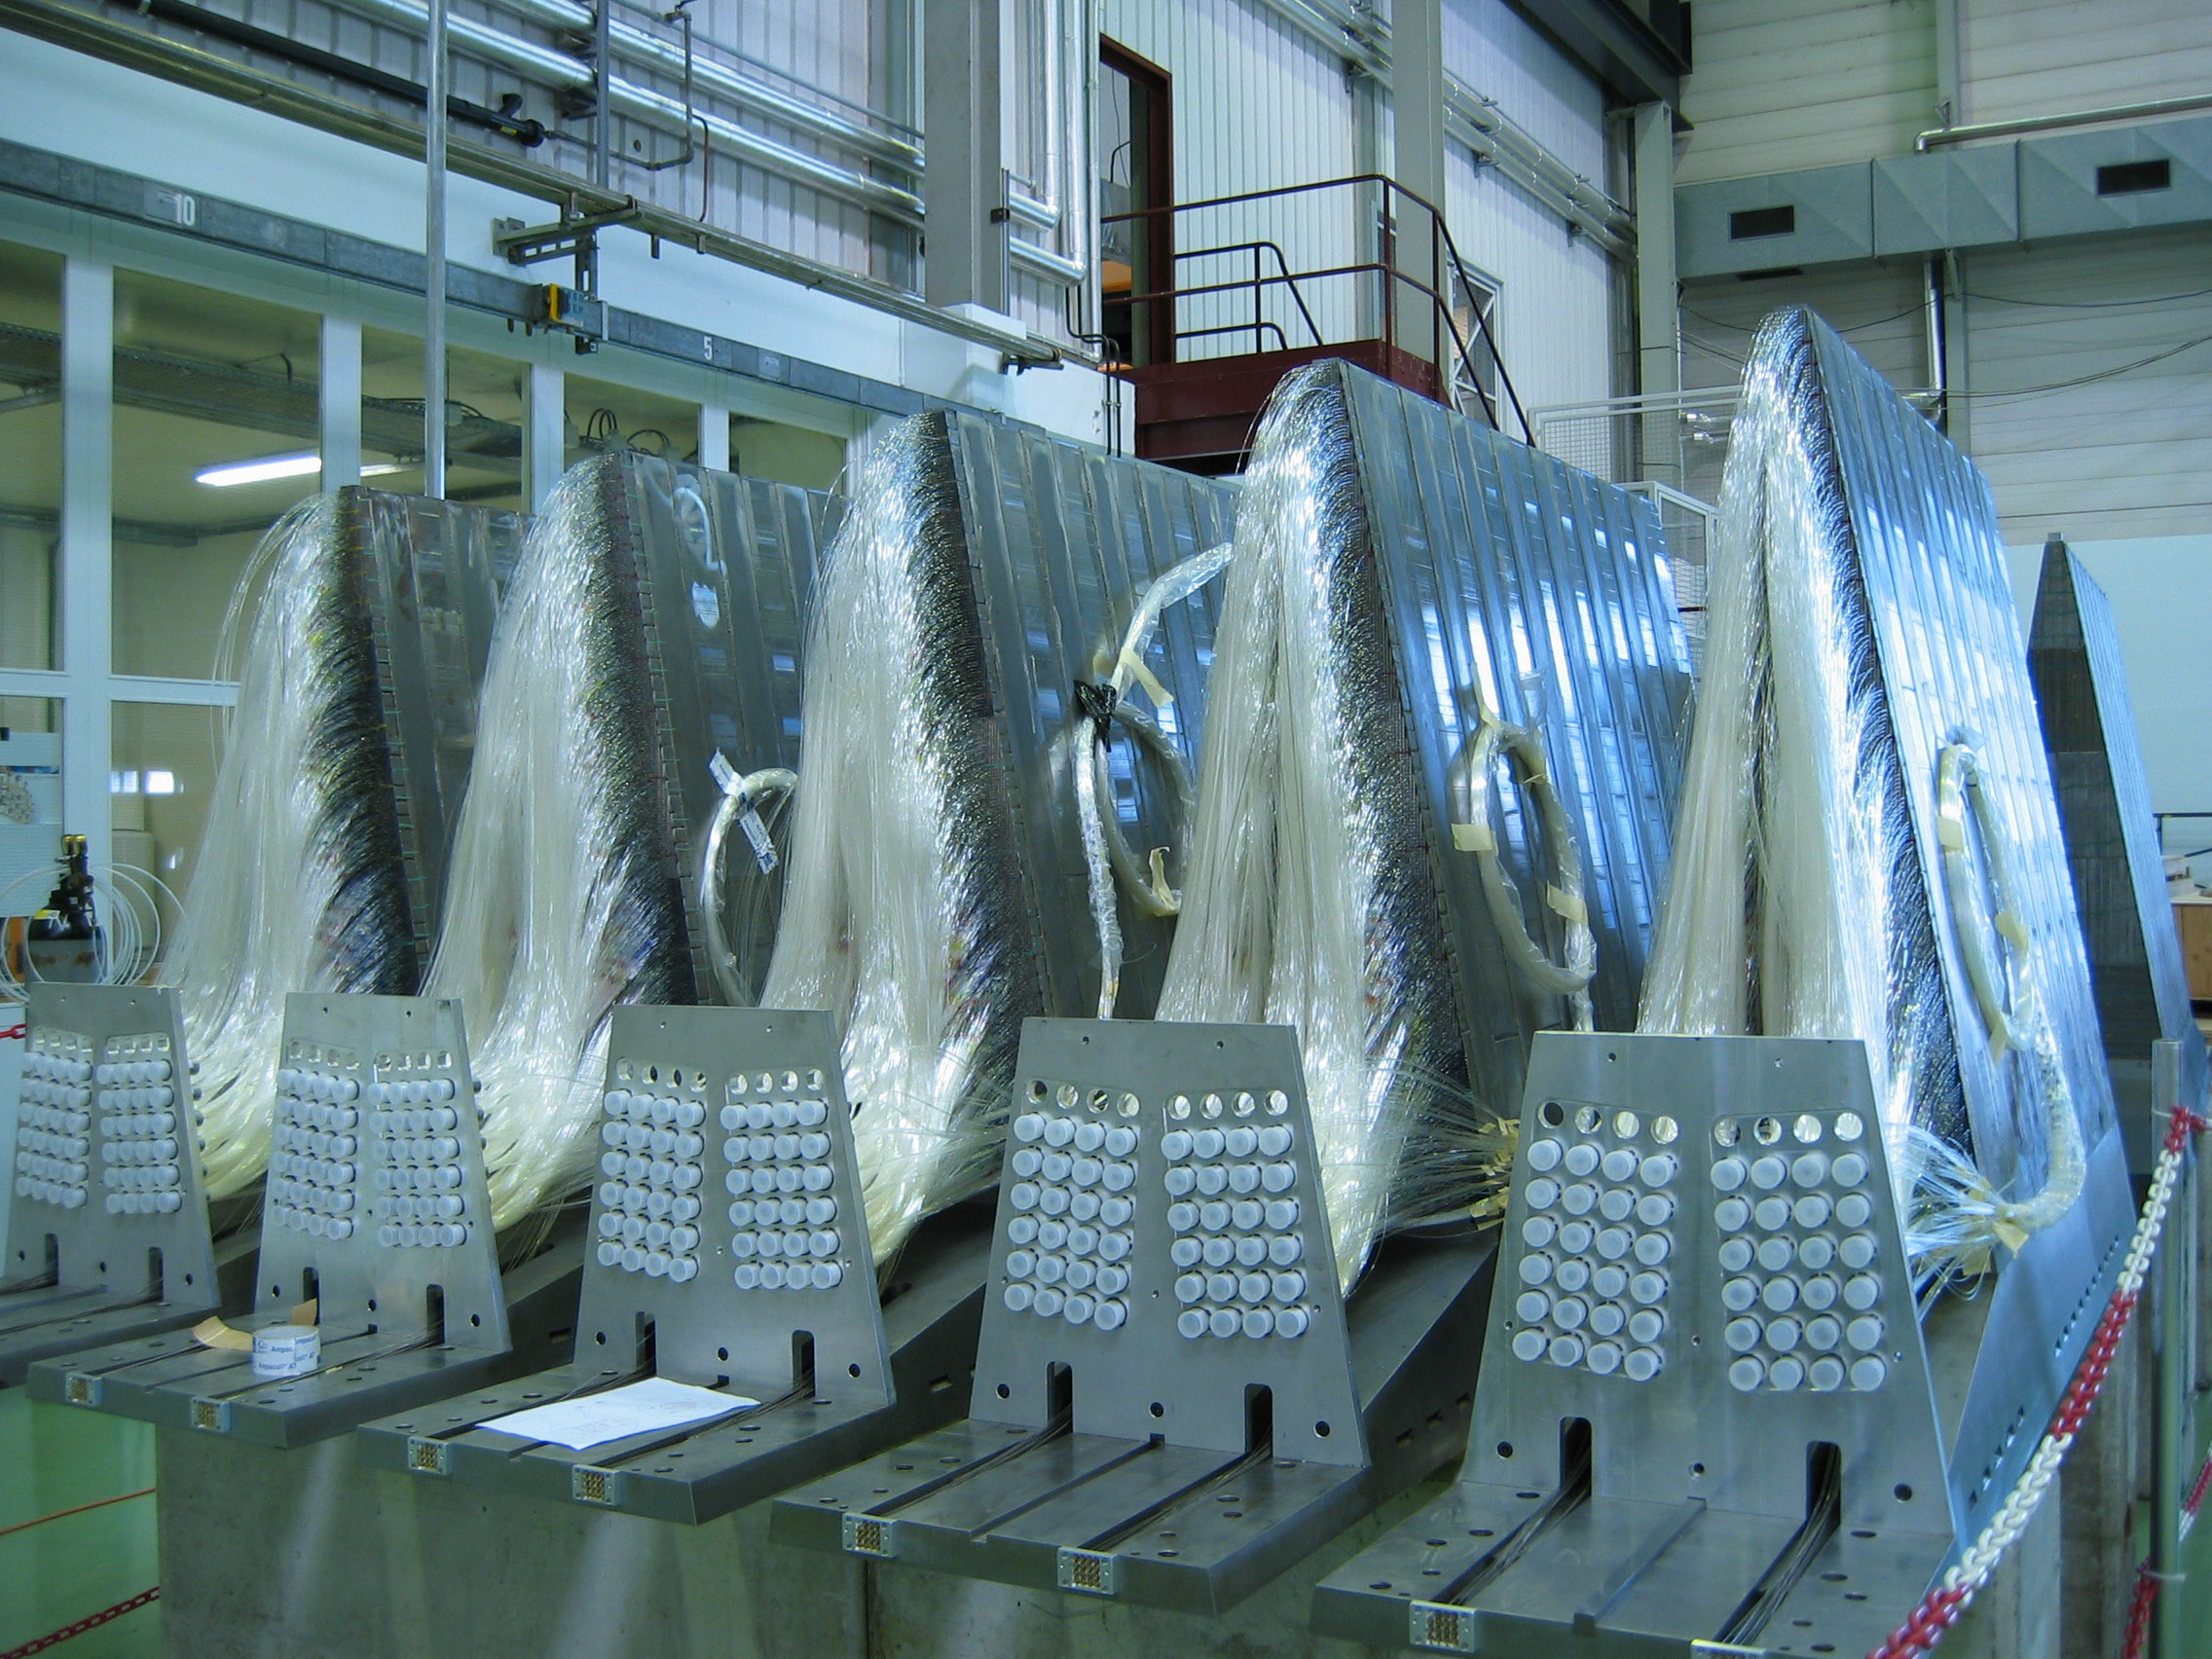
\includegraphics[width=0.98\textwidth]{figures/Ch_4_raddam/HFQuartz.jpg}
				\caption{HF Wedges.}
				\label{figure:HFQuartz}
			\end{center}
		\end{figure}
		%%%%%%%%%%%%%%%%%%%%%%%%%%%%%%%%%%%%%%%%%%
		
		%%%%%%%%%%%%%%%%% HF Tower %%%%%%%%%%%%%%%%%%%
		\begin{figure}[]
			\begin{center}
				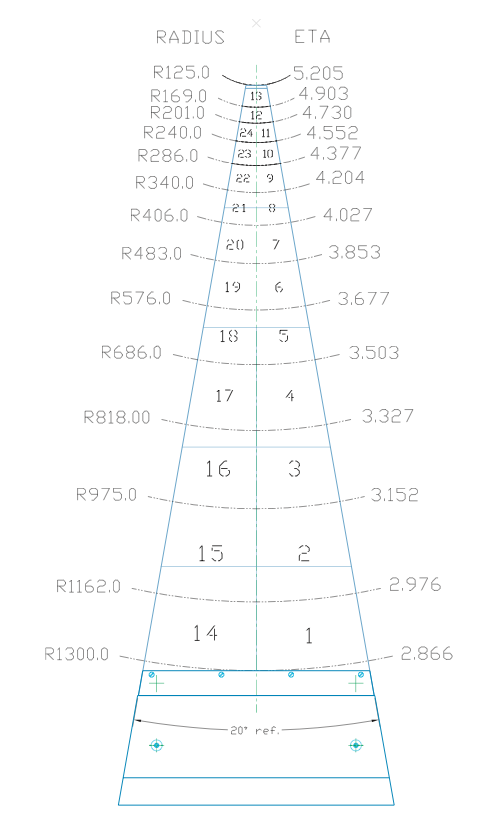
\includegraphics[width=0.5\textwidth]{figures/Ch_4_raddam/HFTowers.png}
				\caption{HF Tower Geometry.}
				\label{figure:HFTower}
			\end{center}
		\end{figure}
		%%%%%%%%%%%%%%%%%%%%%%%%%%%%%%%%%%%%%%%%%%
		
	\section{Radiation Damage in HF}
		The main source of radiation damage to HF will be darkening of the quartz fibers.  This will impact the light transmission of the embedded fibers.  The response of the HF quartz fibers to radiation has been studied in detail at the CERN PS facility IRRAD, see ~\cite{kerem}.  This work resulted in an attenuation formula as a function of delivered dose, up to 1 GRad.  This formula is the crux of the HF radiation damage model:
		%
		\begin{equation}
			I(\lambda,D)/I(\lambda, 0) = \text{exp}[(L/4.343)\alpha(\lambda)(D/D_{s})^{\beta(\lambda)}]\label{eq:attenuation}
		\end{equation}
		This attenuation formula depends on parameters that can have several values, each corresponding to different experimental setups, different fibers, and different wavelengths of light.  In the case of the HF fibers, \(\alpha\) is taken to be 1.44, and \(\beta\) to be 0.44.  This provides the attenuation of a fiber as a function of its absorbed dose.
		%
		Equation \eqref{eq:attenuation} has predicted the observed light attenuation seen by the HF radiation damage online monitoring system very well. Therefore, the radiation damage model built using this formula is expected to give realistic results.
		
		
	\section{Modeling Radiation Damage in HF}		
		\subsection{Implementation}
			The model begins by dividing the HF active area into 100 cells: 10 layers in $r$, and 10 layers in $z$.  Each $z$ layer is 20 cm, and each $r$ layer is 15.75 cm, as shown in Fig. \ref{fig:hfcells}.  Every cell is then assigned a dose variable, calculated using the online calculator linked in \cite{fluka}.  This dose value can be scaled according to the integrated luminosity, as the two quantities are linearly related.  The higher the integrated luminosity passed to the simulation, the higher the doses in the cells.
			
			\begin{figure}[!ht]
				\begin{center}
					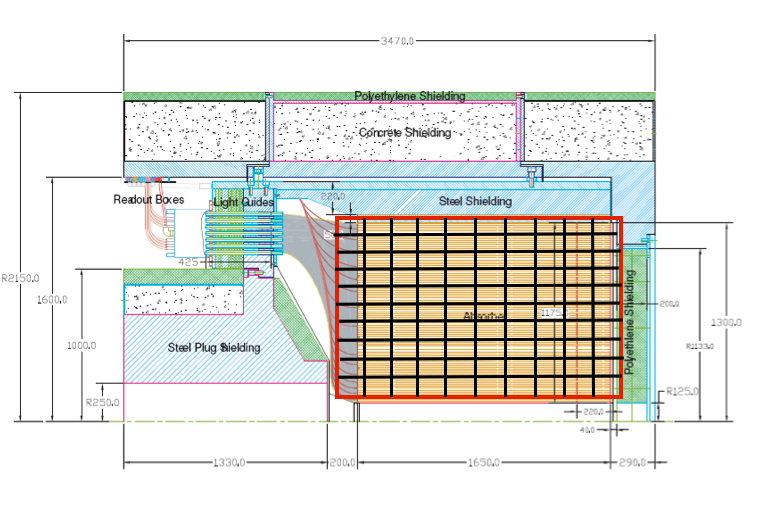
\includegraphics[width=0.98\textwidth]{figures/Ch_4_raddam/DoseMap.png}
					\caption{HF dose map cells.}
					\label{fig:hfcells}
				\end{center}
			\end{figure}
			
			An attenuation factor for each cell is then calculated for a given $(r, z)$ coordinate.  Given the location of the PMT readouts near the rear of HF, and considering that the HF fibers travel along the z-axis parallel to the beam line, the radiation damage model must account for the length of fiber traveled by the Cherenkov light.  If it travels through a short length of fiber, it should be attenuated less, and more if it travels through a long damaged fiber.  The model accounts for this by multiplying together the attenuation factors for each cell, starting from the cell that contains the energy deposit $(r_{\text{hit}}, z_{\text{hit}})$, and ending with the cell at the back of HF $(r_{\text{hit}}, z_{0})$.
			
			The model is implemented into both Fullsim and Fastsim (see Section \ref{section:fullsim}) versions of the HCAL \textit{rechit} simulation package in CMSSW.
		
	\section{Results}
		\subsection{Correction Factors}		
			The light loss calculated by this radiation damage model can be recovered using a recalibration scheme determined from simulation.  The recalibration scheme is a series of parameterizations of correction factors for each $i\eta$ and depth, as a function of integrated luminosity.  The HF detector is segmented in $i\eta$ towers, and each tower has two lengths of fibers, referred to as ``Depth 1" and ``Depth 2", or ``Long" and ``Short", respectively.  The parameterizations are then done for each $i\eta$ and each depth.  
			
			To calculate the correction factors, 2 million pions were generated over the HF $\eta$ range. For each integrated luminosity, in an interval of 500 fb$^{-1}$ from 0 to 10,000 fb$^{-1}$, 100,000 pions were generated using the same MC seed, so only the effects of radiation damage would be considered.  The correction factor is defined as:
			%
			\begin{equation}
				f(i\eta, d, L) = \frac{\sum_{\text{events}} E(i\eta, d, 0)}{\sum_{\text{events}} E(i\eta, d, L)} \label{eq:corr}
			\end{equation}
			%
			In this equation, $E$ is the sum of the energy of the simulated hits for a pion event, $d$ can be 1 (long) or 2 (short) HF fiber, and $L$ is the integrated luminosity in fb$^{-1}$.  A sample of the fits to the correction factors can be reviewed in Figure \ref{fig:hfrecal}.  As expected from numerous CMS radiation dose simulations, the low $\eta$ regions of HF fare the best, and the high $\eta$ regions of HF fare the worst.
			
			\begin{figure}[hbtp]
				\begin{center}
					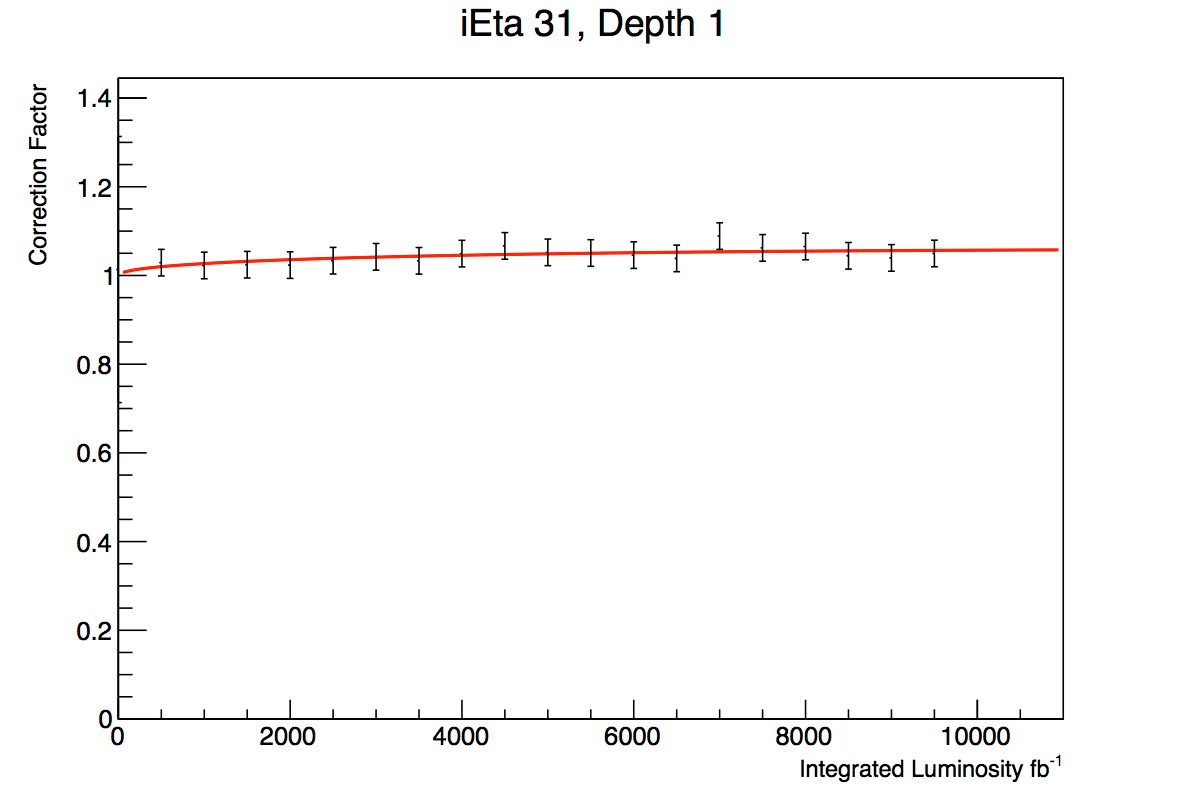
\includegraphics[width=0.49\textwidth]{figures/Ch_4_raddam/HF_31D1.pdf}
					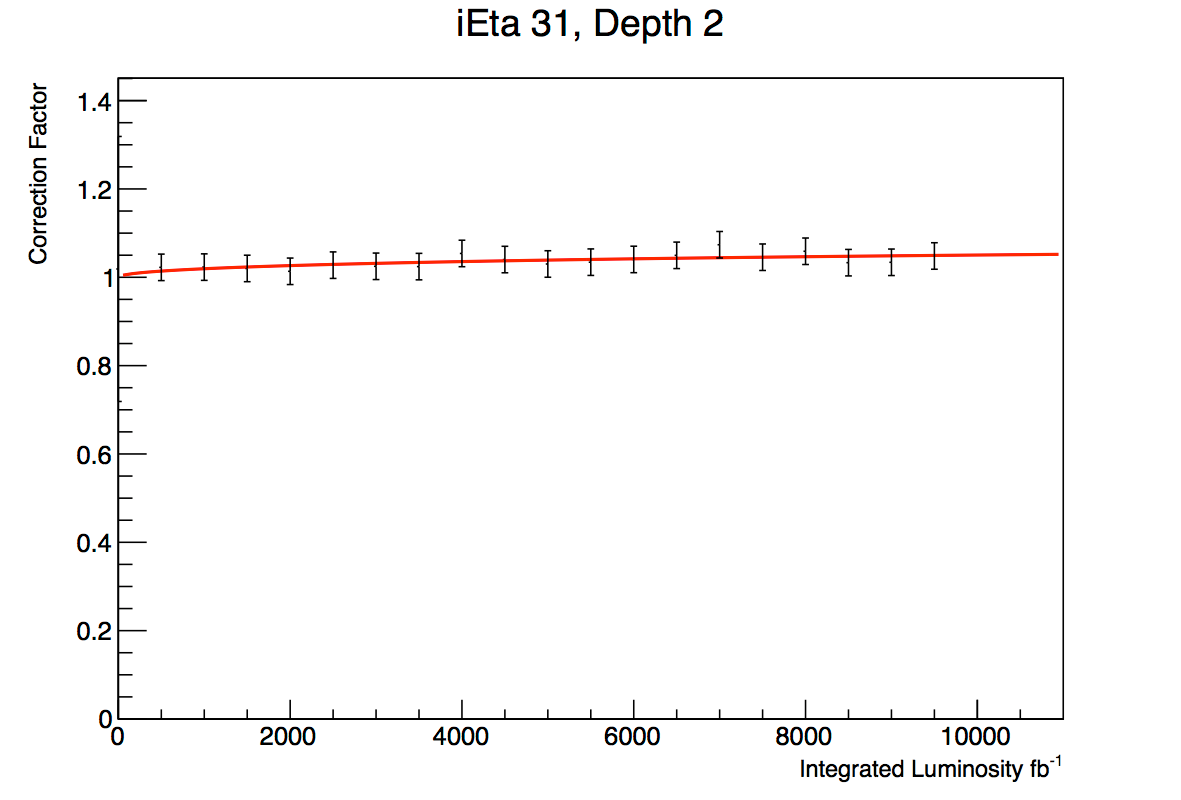
\includegraphics[width=0.49\textwidth]{figures/Ch_4_raddam/HF_31D2.pdf}
					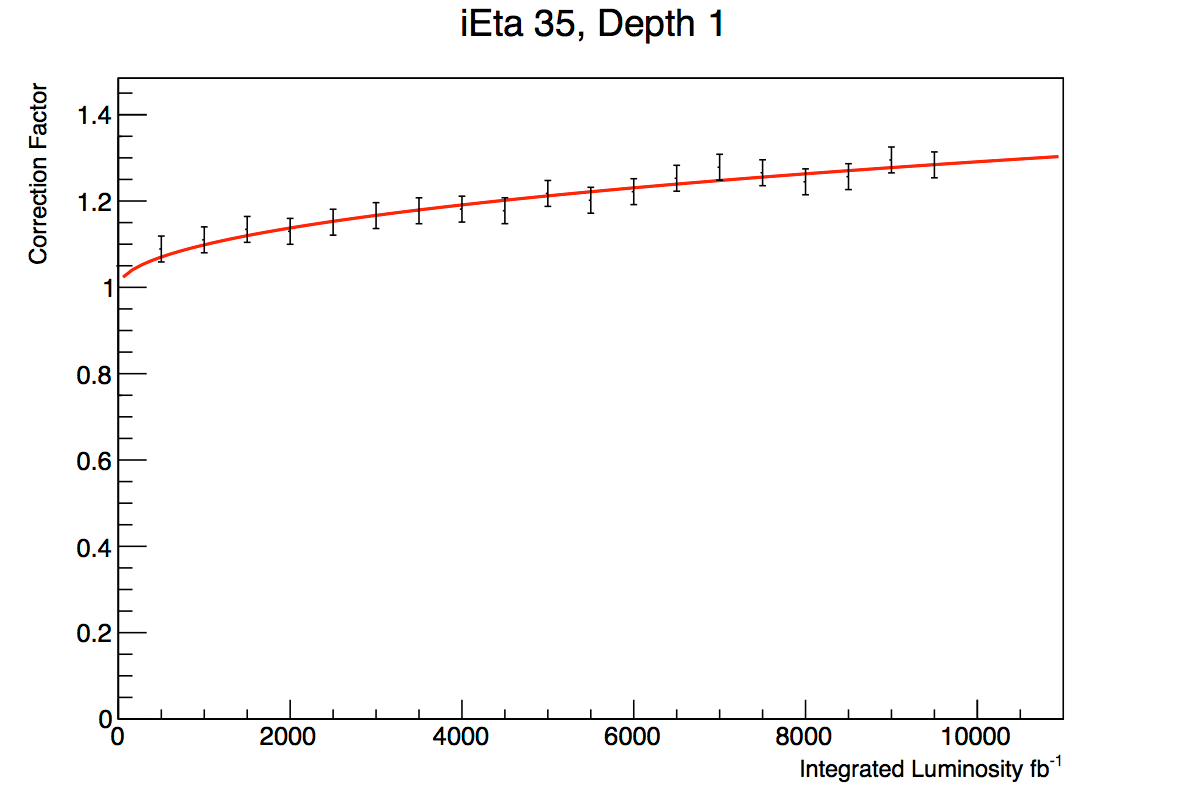
\includegraphics[width=0.49\textwidth]{figures/Ch_4_raddam/HF_35D1.pdf}
					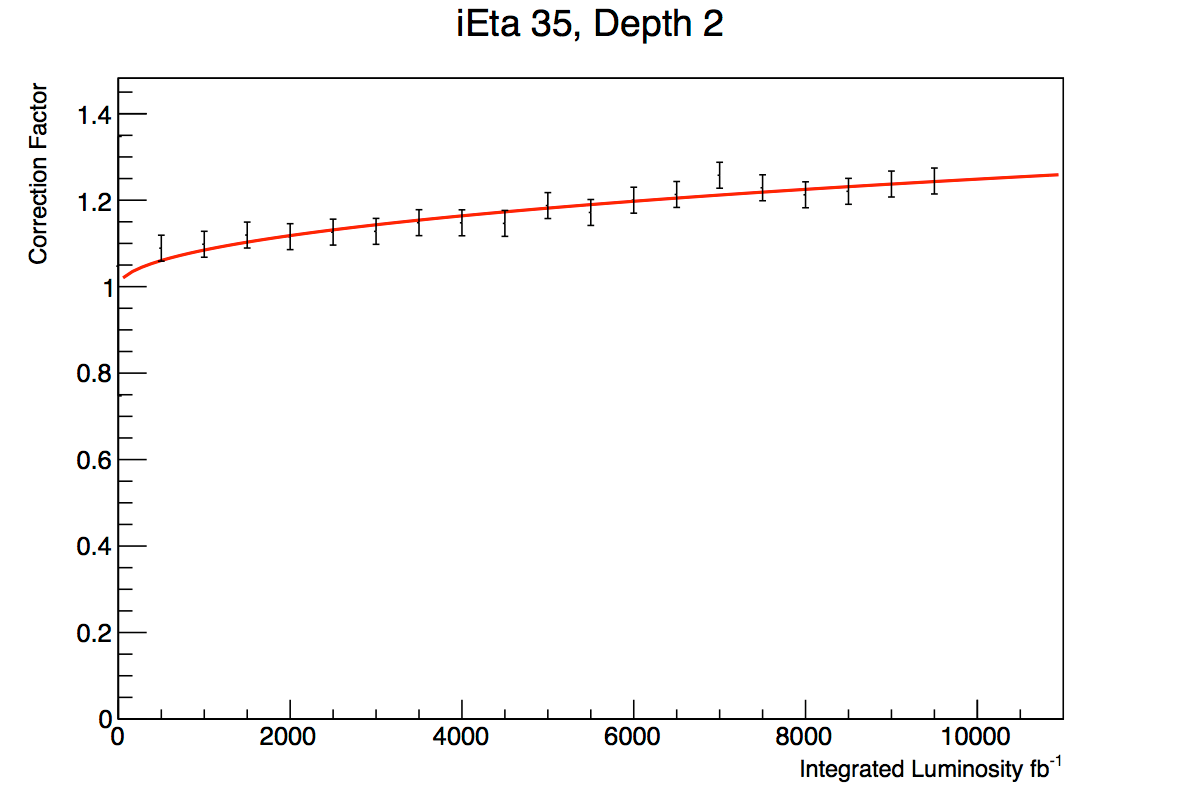
\includegraphics[width=0.49\textwidth]{figures/Ch_4_raddam/HF_35D2.pdf}
					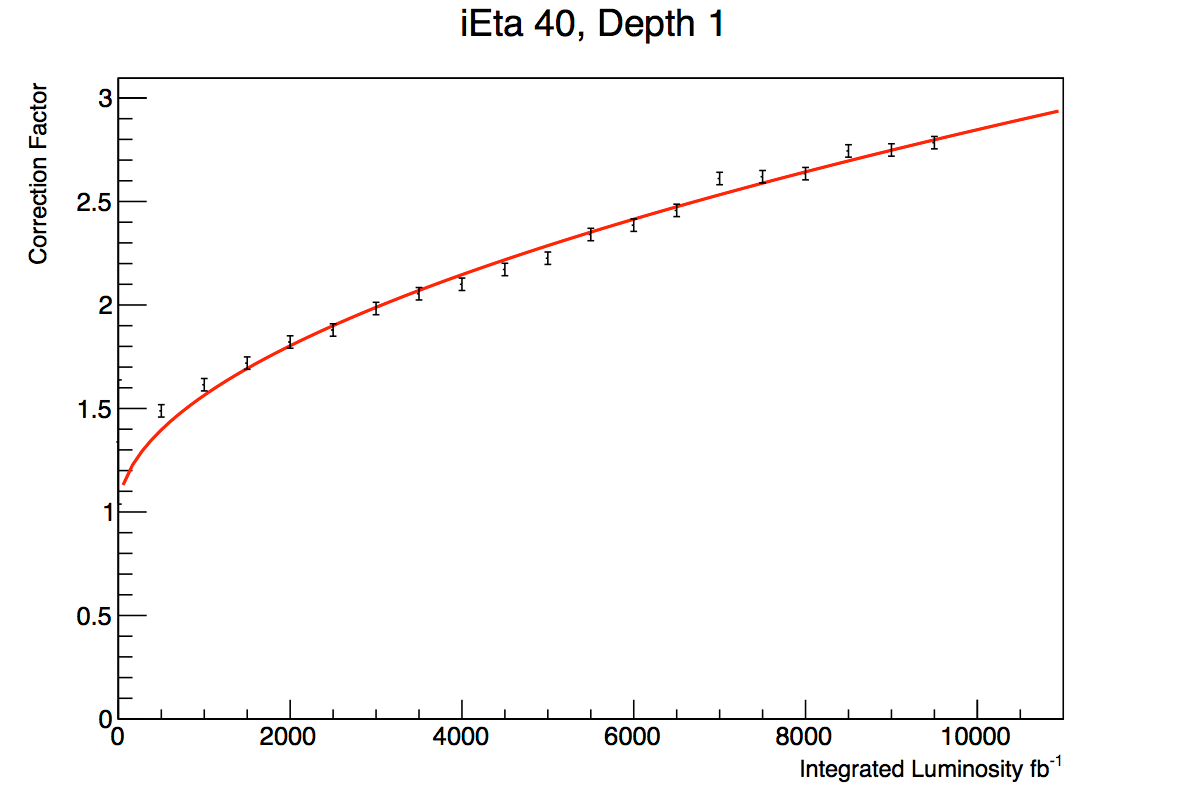
\includegraphics[width=0.49\textwidth]{figures/Ch_4_raddam/HF_40D1.pdf}
					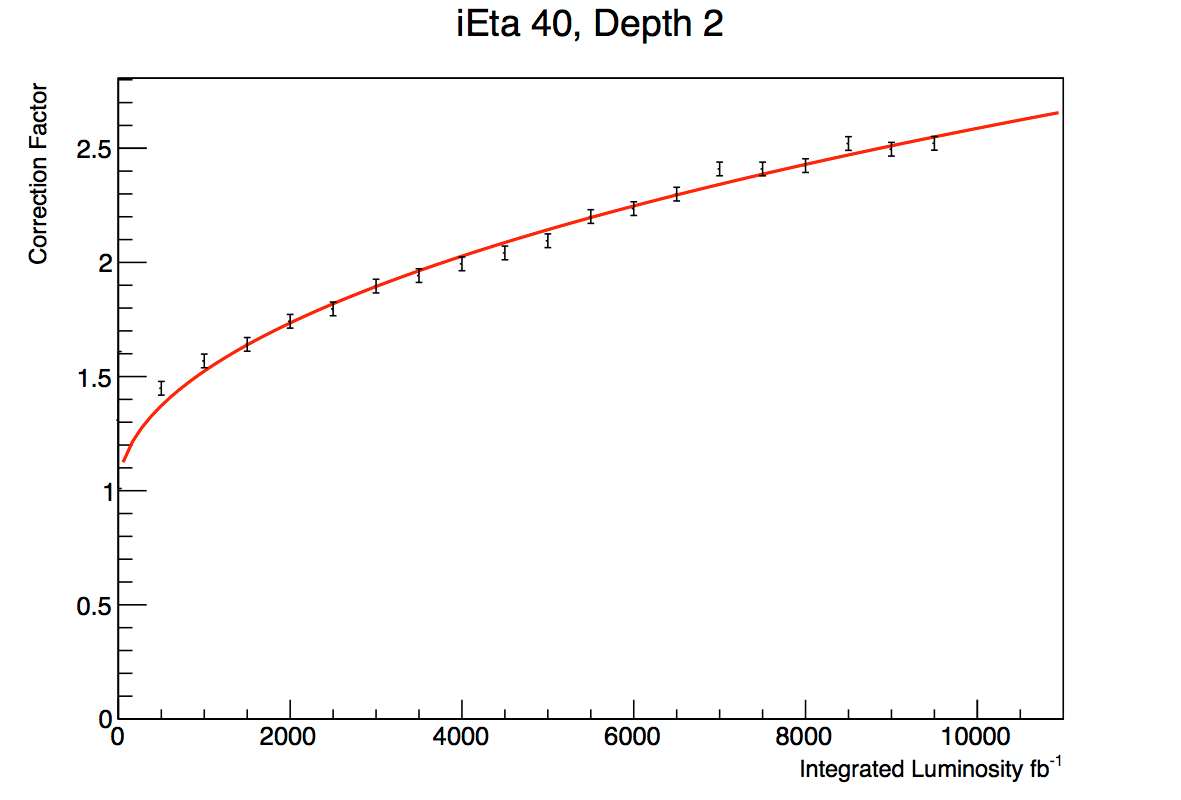
\includegraphics[width=0.49\textwidth]{figures/Ch_4_raddam/HF_40D2.pdf}
					\caption[A sample of HF recalibration parameterizations.]{A sample of HF recalibration parameterizations.  Fits are of the form $1 + A\sqrt{x}+Bx$.}
					\label{fig:hfrecal}
				\end{center}
			\end{figure}
			
		\subsection{Jets in HF}
			To study the effect of damage to the HF fibers on calorimeter jets, 2500 down quarks were generated over the HF $\eta$ range at $L$ = 0, 500, and 3000 fb$^{-1}$.  No pileup was included. The jets were reconstructed with and without energy recalibration enabled.  The jet reconstruction efficiency was defined as:
			%
			\begin{equation}
				\in = \frac{\# \text{calojets matched to genjets}}{\# \text{total number of genjets}}
			\end{equation}
			%
			and was determined by matching the reconstructed calorimeter jets to the generator-level jets. Standard $\Delta R$ matching criteria were used, with $\Delta R < 0.3$, where:
			%
			\begin{equation}
			\Delta R = \sqrt{(\eta_{Calo} - \eta_{Gen})^2+(\phi_{Calo} - \phi_{Gen})^2}
			\end{equation}
			%
			Jets with p$_{T} <$ 30 GeV, or $\eta$ outside the range 3 to 5 were excluded.  The results are shown in Tables \ref{tab:hfJetPtEff} and \ref{tab:hfJetEtaEff}.
			
			\begin{table}
				\centering
				\caption[Efficiencies for varying jet p$_T$ and integrated luminosity for jets from single down quarks in the HF detector.]{Efficiencies for varying jet p$_T$ and integrated luminosity for jets from single down quarks in the HF.}
				\label{tab:hfJetPtEff}
				\begin{center}
					\begin{tabular*}{\textwidth}{@{\extracolsep{\fill}}c c c}
						\hline
						&fb$^{-1}$ & Efficiency (\# Calo Jets / \# Gen Jets) \\ %[0.5ex] % inserts table %heading                                                            
						\hline
						\multicolumn{3}{c}{50 GeV Jets With Recalibration}\\
						&0 & 89.0\% \\
						&500 & 86.5\% \\
						&3000 & 84.0\% \\[1ex]
						\multicolumn{3}{c}{100 GeV Jets No Recalibration}\\
						&0 & 97.4\% \\
						&500 & 97.2\% \\
						&3000 & 95.9\% \\[1ex]
						\multicolumn{3}{c}{100 GeV Jets With Recalibration}\\
						&0 & 97.4\% \\
						&500 & 97.2\% \\
						&3000 & 96.3\% \\[1ex]
						\multicolumn{3}{c}{150 GeV Jets With Recalibration}\\
						&0 & 98.2\% \\
						&500 & 98.5\% \\
						&3000 & 97.8\% \\[1ex]
						\hline
					\end{tabular*}
					\begin{tablenotes}
						\item	Note: Statistical errors are negligible and omitted for brevity.
					\end{tablenotes}	
			    	\end{center}
			\end{table}
			
			\begin{table}
				\centering
				\caption{100 GeV jet efficiency vs. $\eta$.}
				\label{tab:hfJetEtaEff}
				\begin{center}
					\begin{tabular*}{\textwidth}{@{\extracolsep{\fill}}c c c c c}
							\hline
							fb$^{-1}$ &\multicolumn{4}{c}{$|\eta|$ Region}\\
							& 3 - 3.5 & 3.5 - 4 & 4 - 4.5 & 4.5 - 5 \\ [0.5ex]
							\hline
							\multicolumn{5}{c}{No Recalibration}\\
							0 & 100\% & 99.3\% & 98.9\% & 91.1\% \\
							500 & 99.2\% & 99.6\% & 99.0\% & 90.0 \% \\
							3000 & 99.3\% & 98.6\% & 97.8\% & 87.8\% \\
							&&&&\\
							\multicolumn{5}{c}{With Recalibration}\\
							500 & 99.8\% & 99.8\% & 99.1\% & 90.5 \% \\
							3000 & 98.6\% & 99.4\% & 99.5\% & 88.4\% \\
						\hline
					\end{tabular*}
				\begin{tablenotes}
					\item	Note: Statistical errors are negligible and omitted for brevity.
				\end{tablenotes}		
				\end{center}
			\end{table}
			
			\begin{figure}
				\begin{center}
					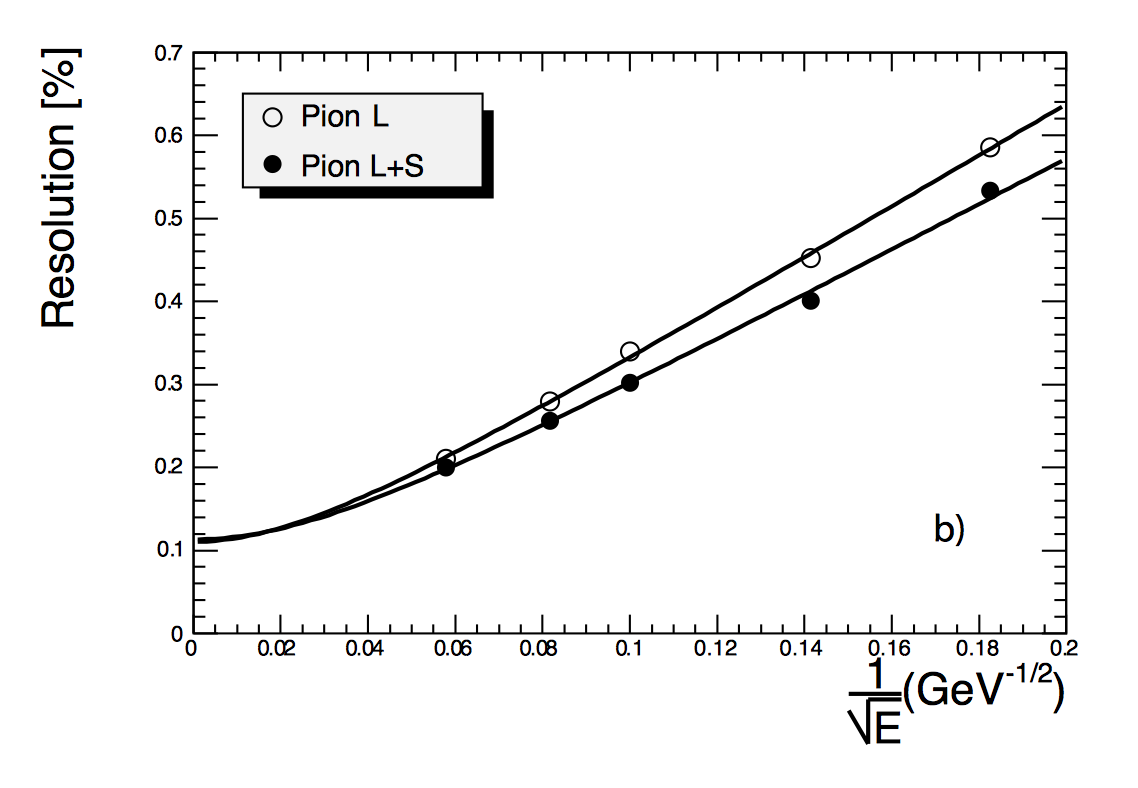
\includegraphics[scale=0.3]{figures/Ch_4_raddam/JetsInHF.png}
					\caption[Energy resolution of the HF detector.]{Energy resolution of the HF detector. \cite{hfresolution}}
					\label{jetsInHF}
				\end{center}
			\end{figure}
		\subsection{Energy Resolution}
			Beyond the scope of this project, and not yet fully determined is how jet energy resolution is affected by radiation damage.  A brief calculation was made for 150 GeV pions at 0 fb$^{-1}$ and 3000 fb$^{-1}$ showing a change in energy resolution of 3.4\% (18.3\% to 21.7\%), which is within the normal operational range of HF, and may be able to be compensated for by the JERC group (JERC is described in Section \ref{JERC}).  Figure \ref{jetsInHF} shows the energy resolution of HF as a function of pion energy as measured in test beam, (without any radiation damage).
		
\section{Conclusion}
A radiation damage simulation was implemented into the official CMSSW release, in both FastSim and FullSim packages.  A performance study of jet reconstruction efficiency in HF was conducted using the FullSim package as a function of integrated luminosity.  The simulation shows that HF will lose some efficiency, however, this loss can be compensated with calibration factors.  The calibration factors were calculated for each tower and depth in HF, and implemented back into the software package with a boolean for easily enabling or disabling both the damage and the calibration.

The outlook is good for HF jet reconstruction efficiency through the entire lifetime of the CMS detector.

\section{Future prospects}
An updated radiation dose map has been created using the FLUKA package.  This new map has better granularity in HF which could lend itself to producing a more accurate simulation.  A new simulation will be implemented using new correction factors calculated with the FLUKA dose map, and results will be compared with the results of this simulation.

Beyond that, a full suite of studies can now be performed using this package by anyone in the CMS collaboration, ensuring robust planning for operating HF well into the future.

